\documentclass[12pt]{article}
\usepackage{lingmacros}
\usepackage{tree-dvips}
\usepackage[a4paper, total={6in, 9in}]{geometry}
\usepackage[parfill]{parskip}
\usepackage{amsmath}
\usepackage{hyperref}
\usepackage{cleveref}
\usepackage{autonum}
\usepackage{amsmath}
\usepackage{pythonhighlight}
\usepackage{graphicx}
\usepackage{caption}
\usepackage{subcaption}
\usepackage[export]{adjustbox}
\graphicspath{ {/home/user/Desktop/LaTeX} }
\begin{document}
\begin{figure}[!tbp]

\section*{\centering{MATH3001: Everything We've Learnt So Far...}}
\medskip 
\subsection*{Chapter 1}
Chapter 1 provides an introduction to Monte Carlo methods, specifically, how we can use randomness to produce accurate results. Random numbers can be used for statistical sampling (also called “Monte Carlo sampling”). A common application of this is in numerical integration. For integration in one dimension, other numerical integration methods (such as Simpson’s and Trapezium rule) are usually more efficient than Monte Carlo Methods. But for multidimensional integrals, Monte Carlo methods become competitive, and for very large numbers of dimensions these are the only practical method for numerical integration.

\subsection*{Homework Task 1}
In Homework Task 1, we used the python code provided in the session to evaluate the mean and variance of a random sample drawn from probability distributions.
\medskip 
\medskip 

  \begin{subfigure}[b]{0.4\textwidth}
    \includegraphics[width=\textwidth]{Normal_1000.png}
    \caption{$N$ = $1,000$}
    \label{fig:f1}
  \end{subfigure}
  \hfill
  \begin{subfigure}[b]{0.41\textwidth}
    \includegraphics[width=\textwidth]{Normal_10000.png}
    \caption{$N$ = $10,000$}
    \label{fig:f2}
  \end{subfigure}
  \caption{Random Sampling from a Normal Distribution}
\end{figure}

In Figure 1, we see that as you increase the value of $N$, the closer to the Normal Distribution the random sampling is. Like the Law of Large Numbers, this is a phenomenon we expect. 

We can analyse how good these random sampling approximations of the mean and variance are. First, we will plot the approximations of the mean for different values of N for both the exponential and normal distributions, as can be seen in Figure 2. 

We observe that, even for $N = 100,000$, the Normal Distribution and Exponential Distribution do not calculate the exact value for the mean. In particular, we see that the Exponential Distribution is actually better at estimating the true value of the mean when compared to the Normal Distribution. 

Although these distributions do not give an output that is the exact mean, we can incorporate percentage values and consider for what values of N we need to be within a particular percentage of the mean. 

\begin{figure}[h!]
  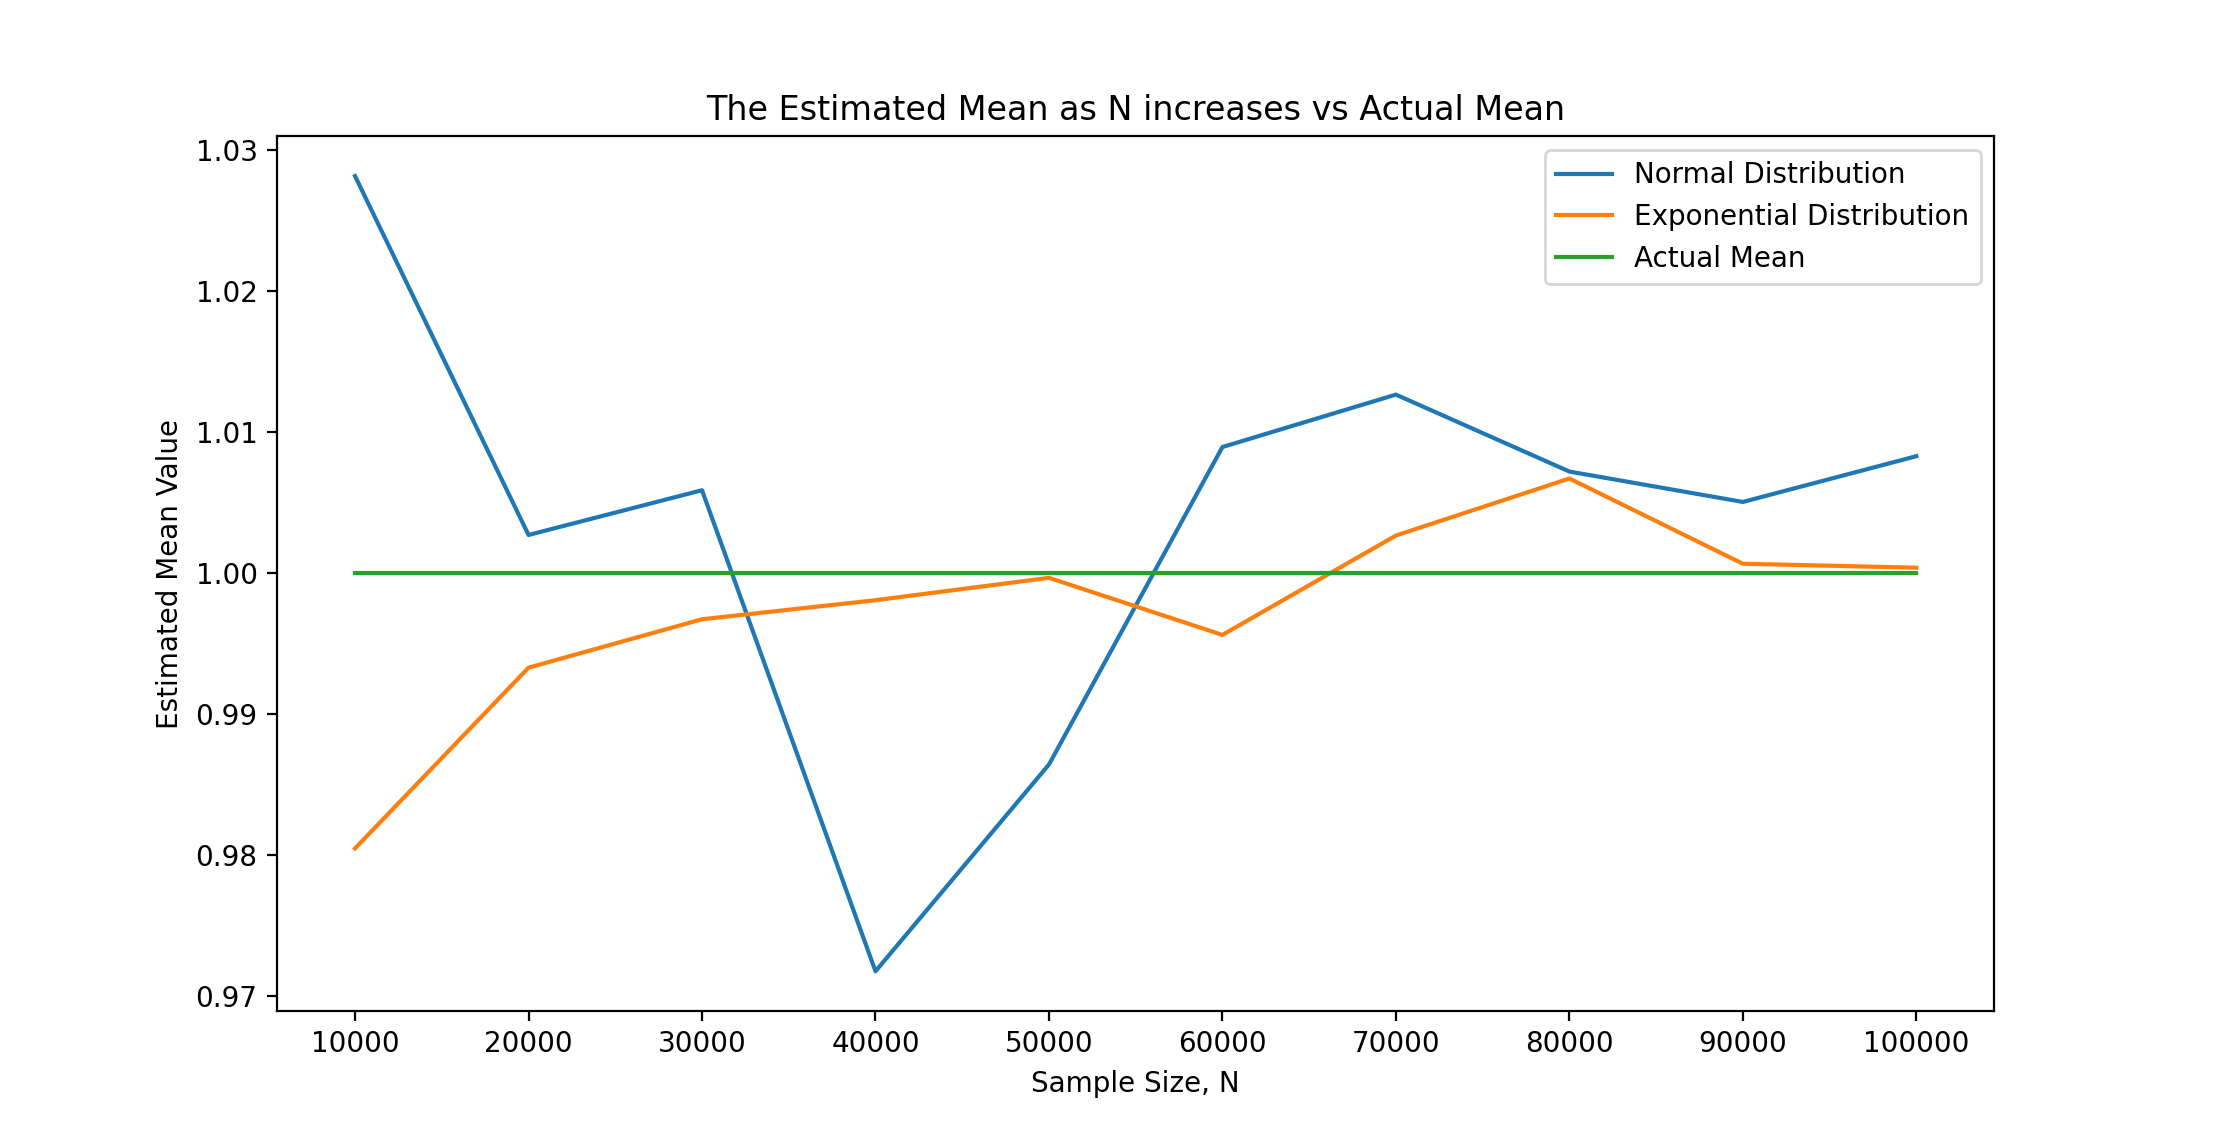
\includegraphics[scale=0.45, center]{Estimated Mean, 10,000 to 100,000}
  \caption{Estimated Mean as N Increases vs Actual Mean}
  \label{fig:estimated_mean}
\end{figure}

In Figure 3, we observe the effect of estimating the mean within a percentage value, as can be seen by the red lines. In this example, we used a 5 percent error estimation for the Normal Distribution and Exponential Distribution.

\begin{figure}[h]
\begin{subfigure}{0.5\textwidth}
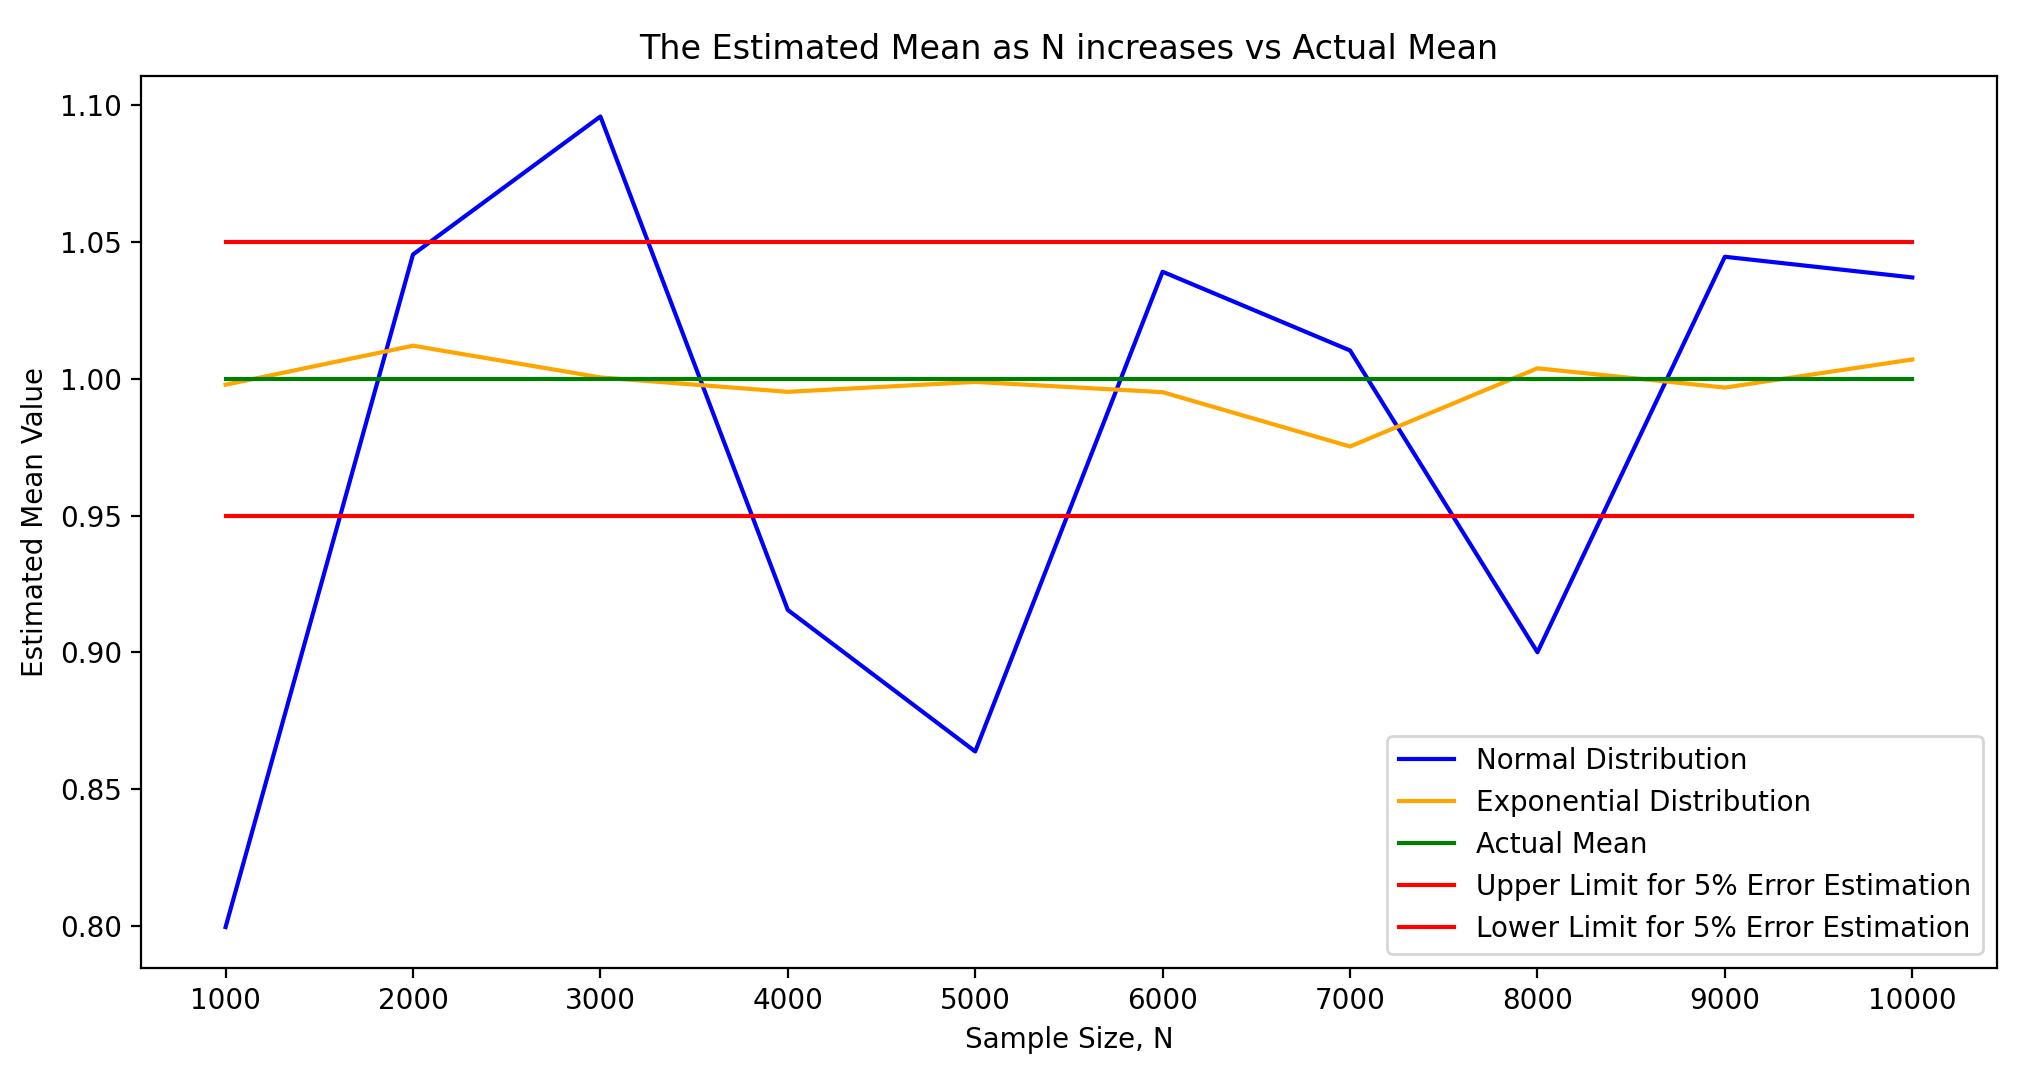
\includegraphics[width=1\linewidth, left]{1,000 to 10,000 5 percent error.png} 
\caption{$N = 10,000$}
\label{fig:subim1}
\end{subfigure}
\begin{subfigure}{0.5\textwidth}
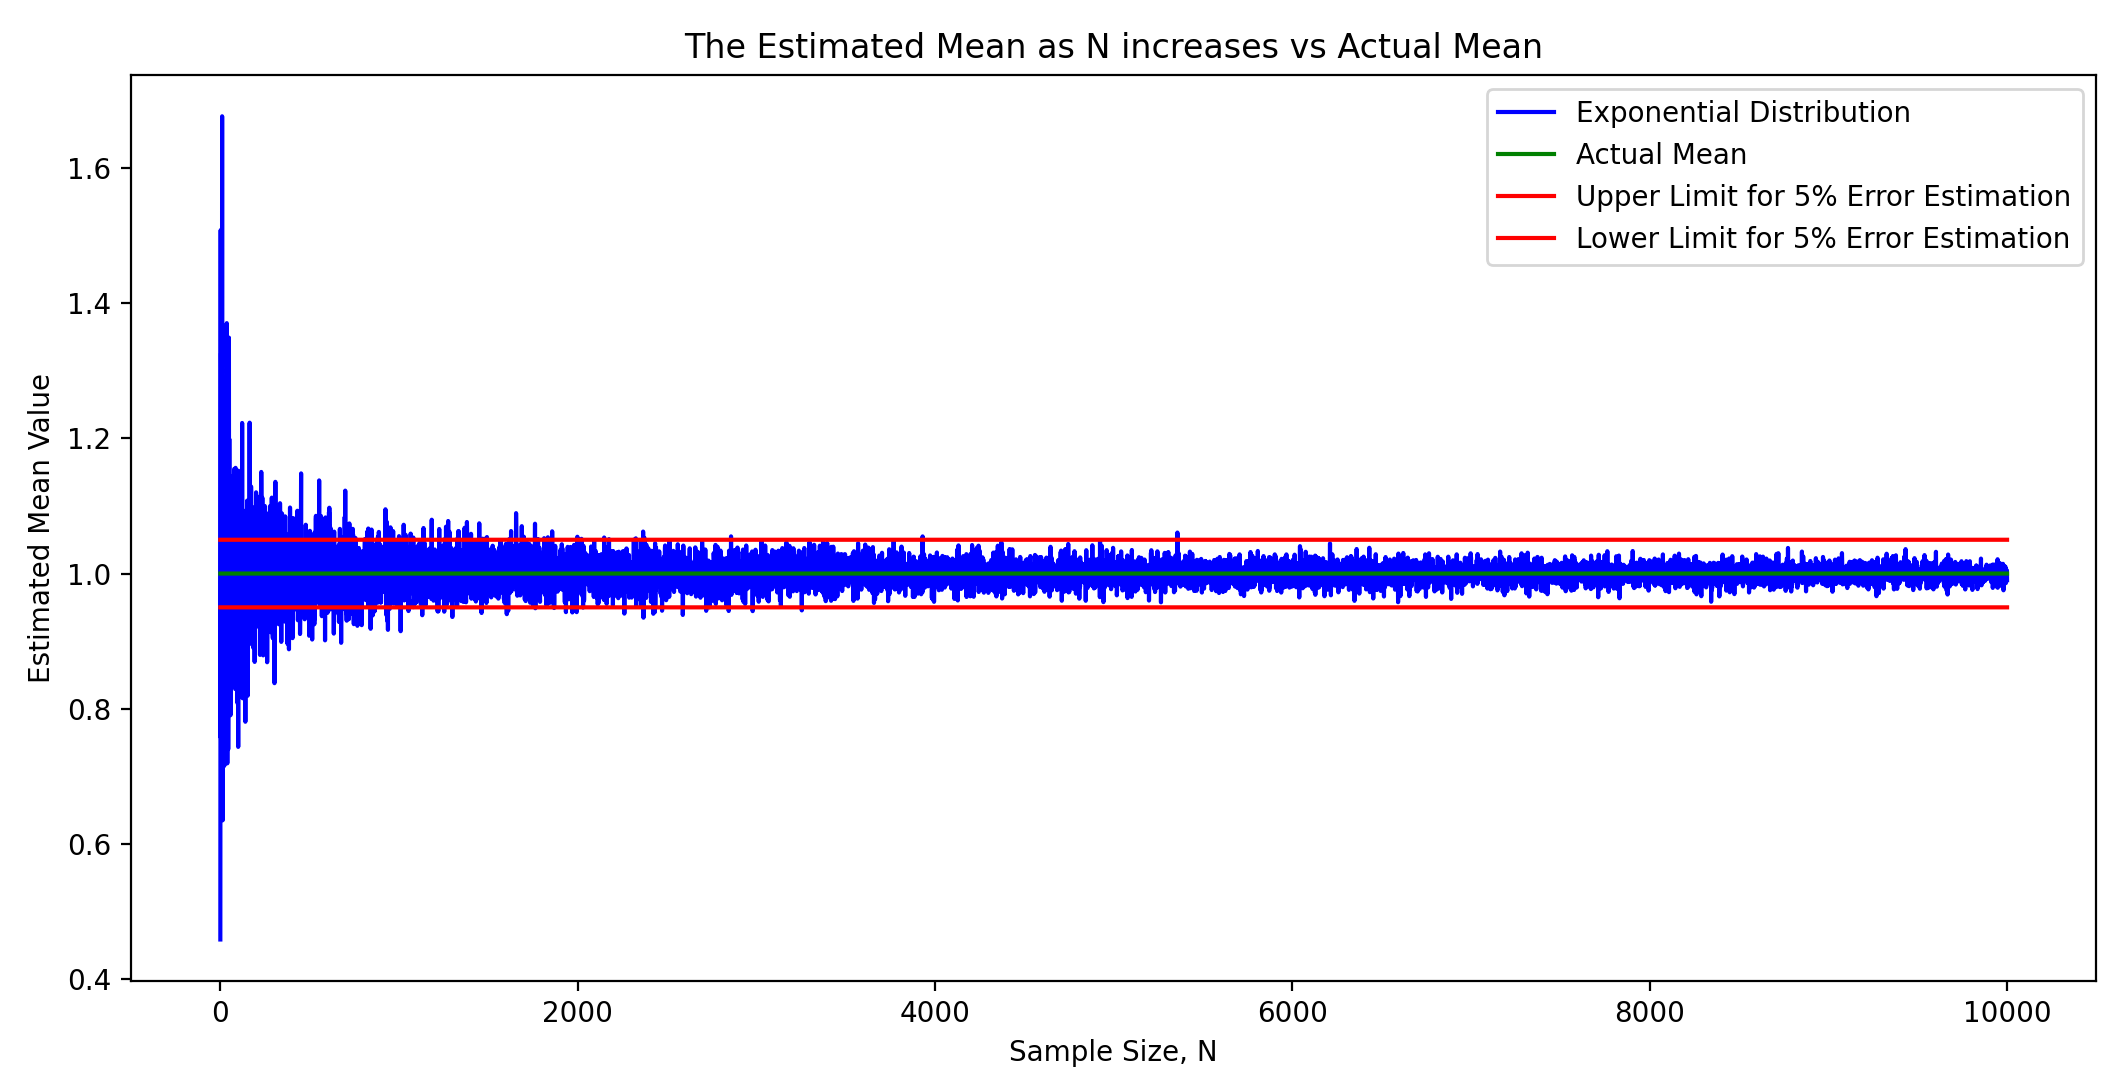
\includegraphics[width=1.03\linewidth]{Exponential N = 10,000.png}
\caption{$N = 1,000,000$}
\label{fig:subim2}
\end{subfigure}
\caption{Estimated Mean Within a Percentage Range}
\label{fig:image2}
\end{figure}

It is clear that as N is increased, the estimated mean lies within the upper and lower limit of the percentage error estimation. Although this is intuitive, it allows us to consider the standard error of the mean and then observe what minimum N value we need to be within a particular error percentage. 

We now consider the standard error of the mean, which can be defined as:
\begin{align}
\sigma\textsubscript{$\langle x\rangle$\textsubscript{$N$}}  = \frac{\sigma\textsubscript{$x$}}{\sqrt{N}}
\end{align}
where $N$ is the number of samples, $\sigma\textsubscript{$x$}$ is the actual mean and $\langle x\rangle\textsubscript{$N$}$ is the estimated mean for $N$ samples.

We can now plot the standard error of the mean for different distributions and increasing values of N. As can be seen in Figure 4. 
 
\begin{figure}[h!]
  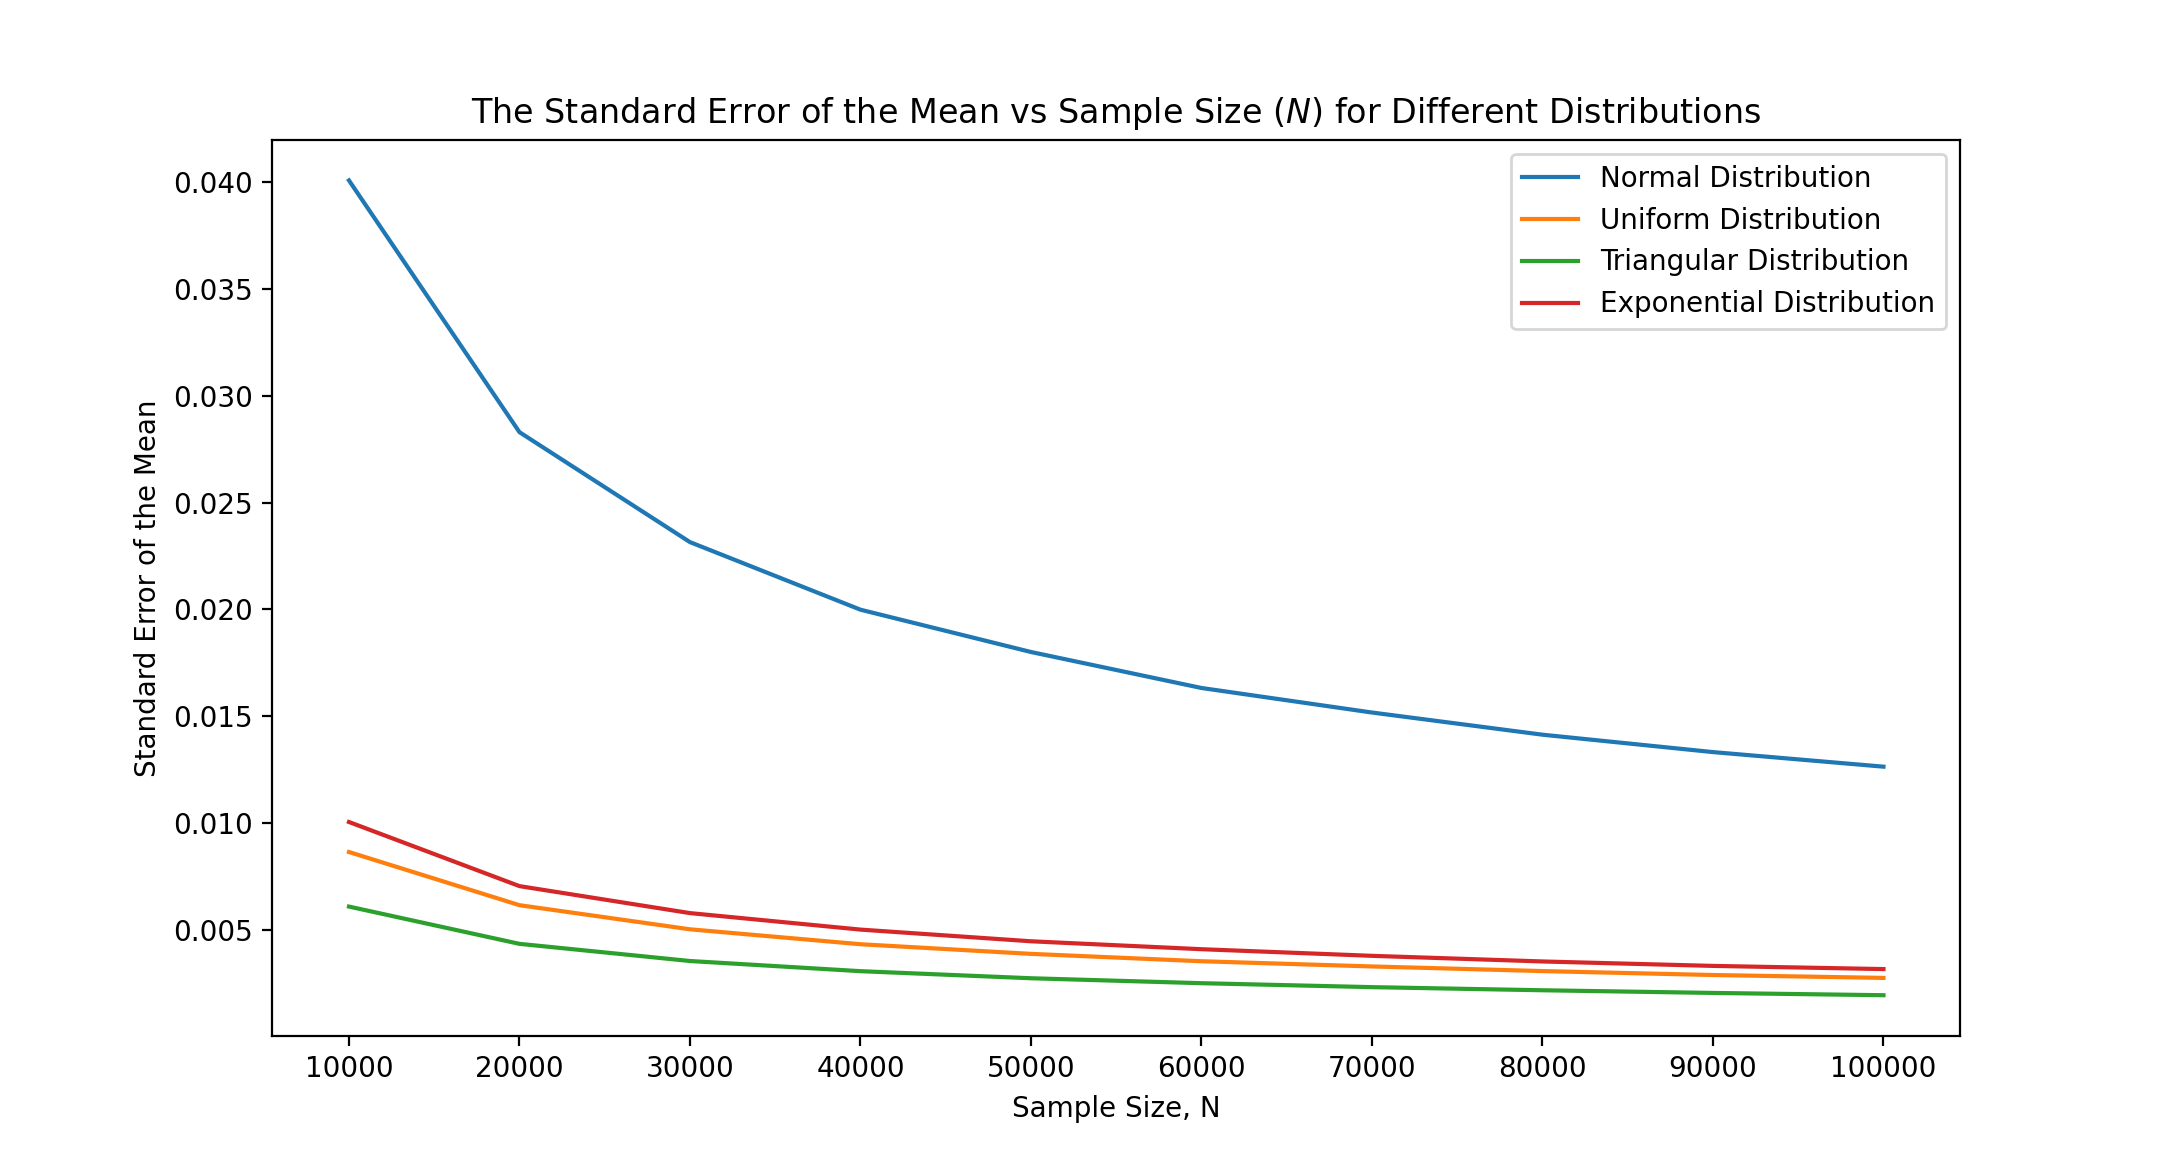
\includegraphics[scale=0.45, center]{10,000 to 100,000.png}
  \caption{Standard Error of the Mean for Different Distributions}
  \label{fig:estimated_mean}
\end{figure}

These distributions each have different parameters which gives rise to the different convergence rates. Again, we notice that as we increase N, the standard error of the mean decreases. 

We can use the standard error of the mean formula to calculate the minimum value of $N$ needed for the estimate to lie within a percentage of the true mean.

\subsubsection*{An Example}
Let's say we have \[
  X \sim \mathcal{N}(0,1)\,.
\]
What is the minimum value of $N$ needed for our estimated mean to be within a 0.5 percent standard error of the actual mean?

Rearranging the formula for the standard error of the mean, we have 
 

\begin{align}
N  &= (\frac{\sigma\textsubscript{$x$}}{\sigma\textsubscript{$\langle x\rangle$\textsubscript{$N$}}})^2\\\\
&= (\frac{1}{0.005})^2 \\\\
&= 40,000
\end{align}

Thus, the minimum value of $N$ needed to ensure our estimated mean would be within a 0.5 percent standard error of the mean is $N = 40,000$!

\subsection*{Chapter 2}
\subsection*{Monte Carlo Integration}

In Chapter 2, we extend Monte Carlo methods to look at integration. We then compare these methods with other quadrature methods like the Simpson's Rule and the Trapezium Rule. 

In Monte Carlo integration, the points are chosen randomly from a distribution. Since the mean value of f can be defined as
\begin{equation}
\langle f\rangle = \frac{1}{b-a}\int_{a}^{b} f(x) \,dx 
\end{equation}

we can determine the value of the integral by sampling f to find its mean value. Thus if we draw $N$ points,  $x\textsubscript{$1$}$,... $x\textsubscript{$N$}$ from a uniform distribution in the interval [a, b] then we can estimate the integral as,
\begin{equation}
\int_{a}^{b} f(x) \,dx \approx \frac{(b-a)}{N}\sum_{i=1}^{N} f(x_{i})\,
\end{equation}

Furthermore we can also estimate the error, by taking the square root of the mean
squared error as
 \begin{align} 
\frac{(b-a)}{\sqrt{N}}\sigma
\end{align}

where $\sigma^2$ is the variance of $f$ over the interval. This means that the accuracy of the estimate improves as the square root of the number of points sampled.

\subsection*{Multi-dimensional Integration}

As will be seen in the following answers to the Homework Tasks, there are better ways of integrating in one-dimension than Monte-Carlo (MC) methods.

In the notes, there is a comment on quadrature schemes for multi-dimensional examples. The consensus is that for the Simpson's Rule and Trapezium Rule, the total error will scale as $N^\frac{-1}{D}$. So when $D$ is large, the convergence is very slow. Even where we have a rectangular domain over which the function is differentiable the convergence rate we decrease as the number of dimensions increases. This is the “curse of dimensionality”.

For Monte Carlo Sampling:

The integral can be estimated as,
 \begin{align} 
\int\limits_V f(\mathbf{x}) \, dx \approx \frac{V}{N}\sum_{i=1}^{N} f(\mathbf{x}_{i})\, \pm V\frac{\sigma}{\sqrt{N}}
\end{align}

Hence, the error scales as $N^{\frac{-1}{2}}$ irrespective of the number of dimensions. 

\subsection*{Homework Task 2 (i)}

For a general function $f(x)$ obtain a formula for $\sigma$ and hence an error estimate.

\subsubsection*{Answer}

From the provided notes, we define the mean of a function $f(x)$,  $\langle f\rangle$ as:
\begin{equation}
\langle f\rangle = \frac{1}{b-a}\int_{a}^{b} f(x) \,dx 
\end{equation}
By intuition, we can deduce:
\begin{equation}
\langle f\rangle ^2 = \frac{1}{b-a}\int_{a}^{b} f(x)^2 \,dx 
\end{equation}

It is clear to see that the formula for $\sigma$ is:
\begin{equation}
\sigma =  \sqrt{{\langle f\rangle} - {\langle f\rangle ^2}}
\end{equation}

Using these results, it is easy to see that an unbiased estimate for the standard deviation of the random integration, $\sigma\textsubscript{$\langle f\rangle$\textsubscript{$N$}}$, (which is also denoted as the standard error component while using Monte Carlo integration), is the following:

\begin{equation}
\sigma\textsubscript{$\langle f\rangle$\textsubscript{$N$}} = \sqrt{\frac{
\langle f\rangle - \langle f\rangle ^2 }{N}}
\end{equation}

This is the formula for the error estimate. 

\subsection*{Homework Task 2 (ii)}

How does this compare with quadrature schemes such as the trapezium rule or Simpson’s rule? Write a program to estimate $\frac{1}{2}\int_{0}^{2} cos^2(x) \,dx$ using Monte-Carlo sampling. Compare the answer with the trapezium and/or Simpson’s rule. Is Monte-Carlo sampling a good way to estimate this integral?

\subsubsection*{Answer}

For most of the 1D integration, the quadrature schemes such as Simpson's Rule and Trapezium Rule perform better than the Monte Carlo method. For integration, the Monte Carlo method is usually used for high dimensional cases, like 3D integration or even higher than 3D. \par

Now, we use Monte Carlo Integration to solve the following integral,
\begin{align}
I = \frac{1}{2}\int_{0}^{2} cos^2(x) \,dx
\end{align}

We have produced code in Python that allows us to accurately estimate this integral using Monte Carlo methods. Below is a visual representation of $N$ = 1000 individual estimates. It is worth including this graph as it represents the randomness of these estimates. 
 
\begin{figure}[h!]
  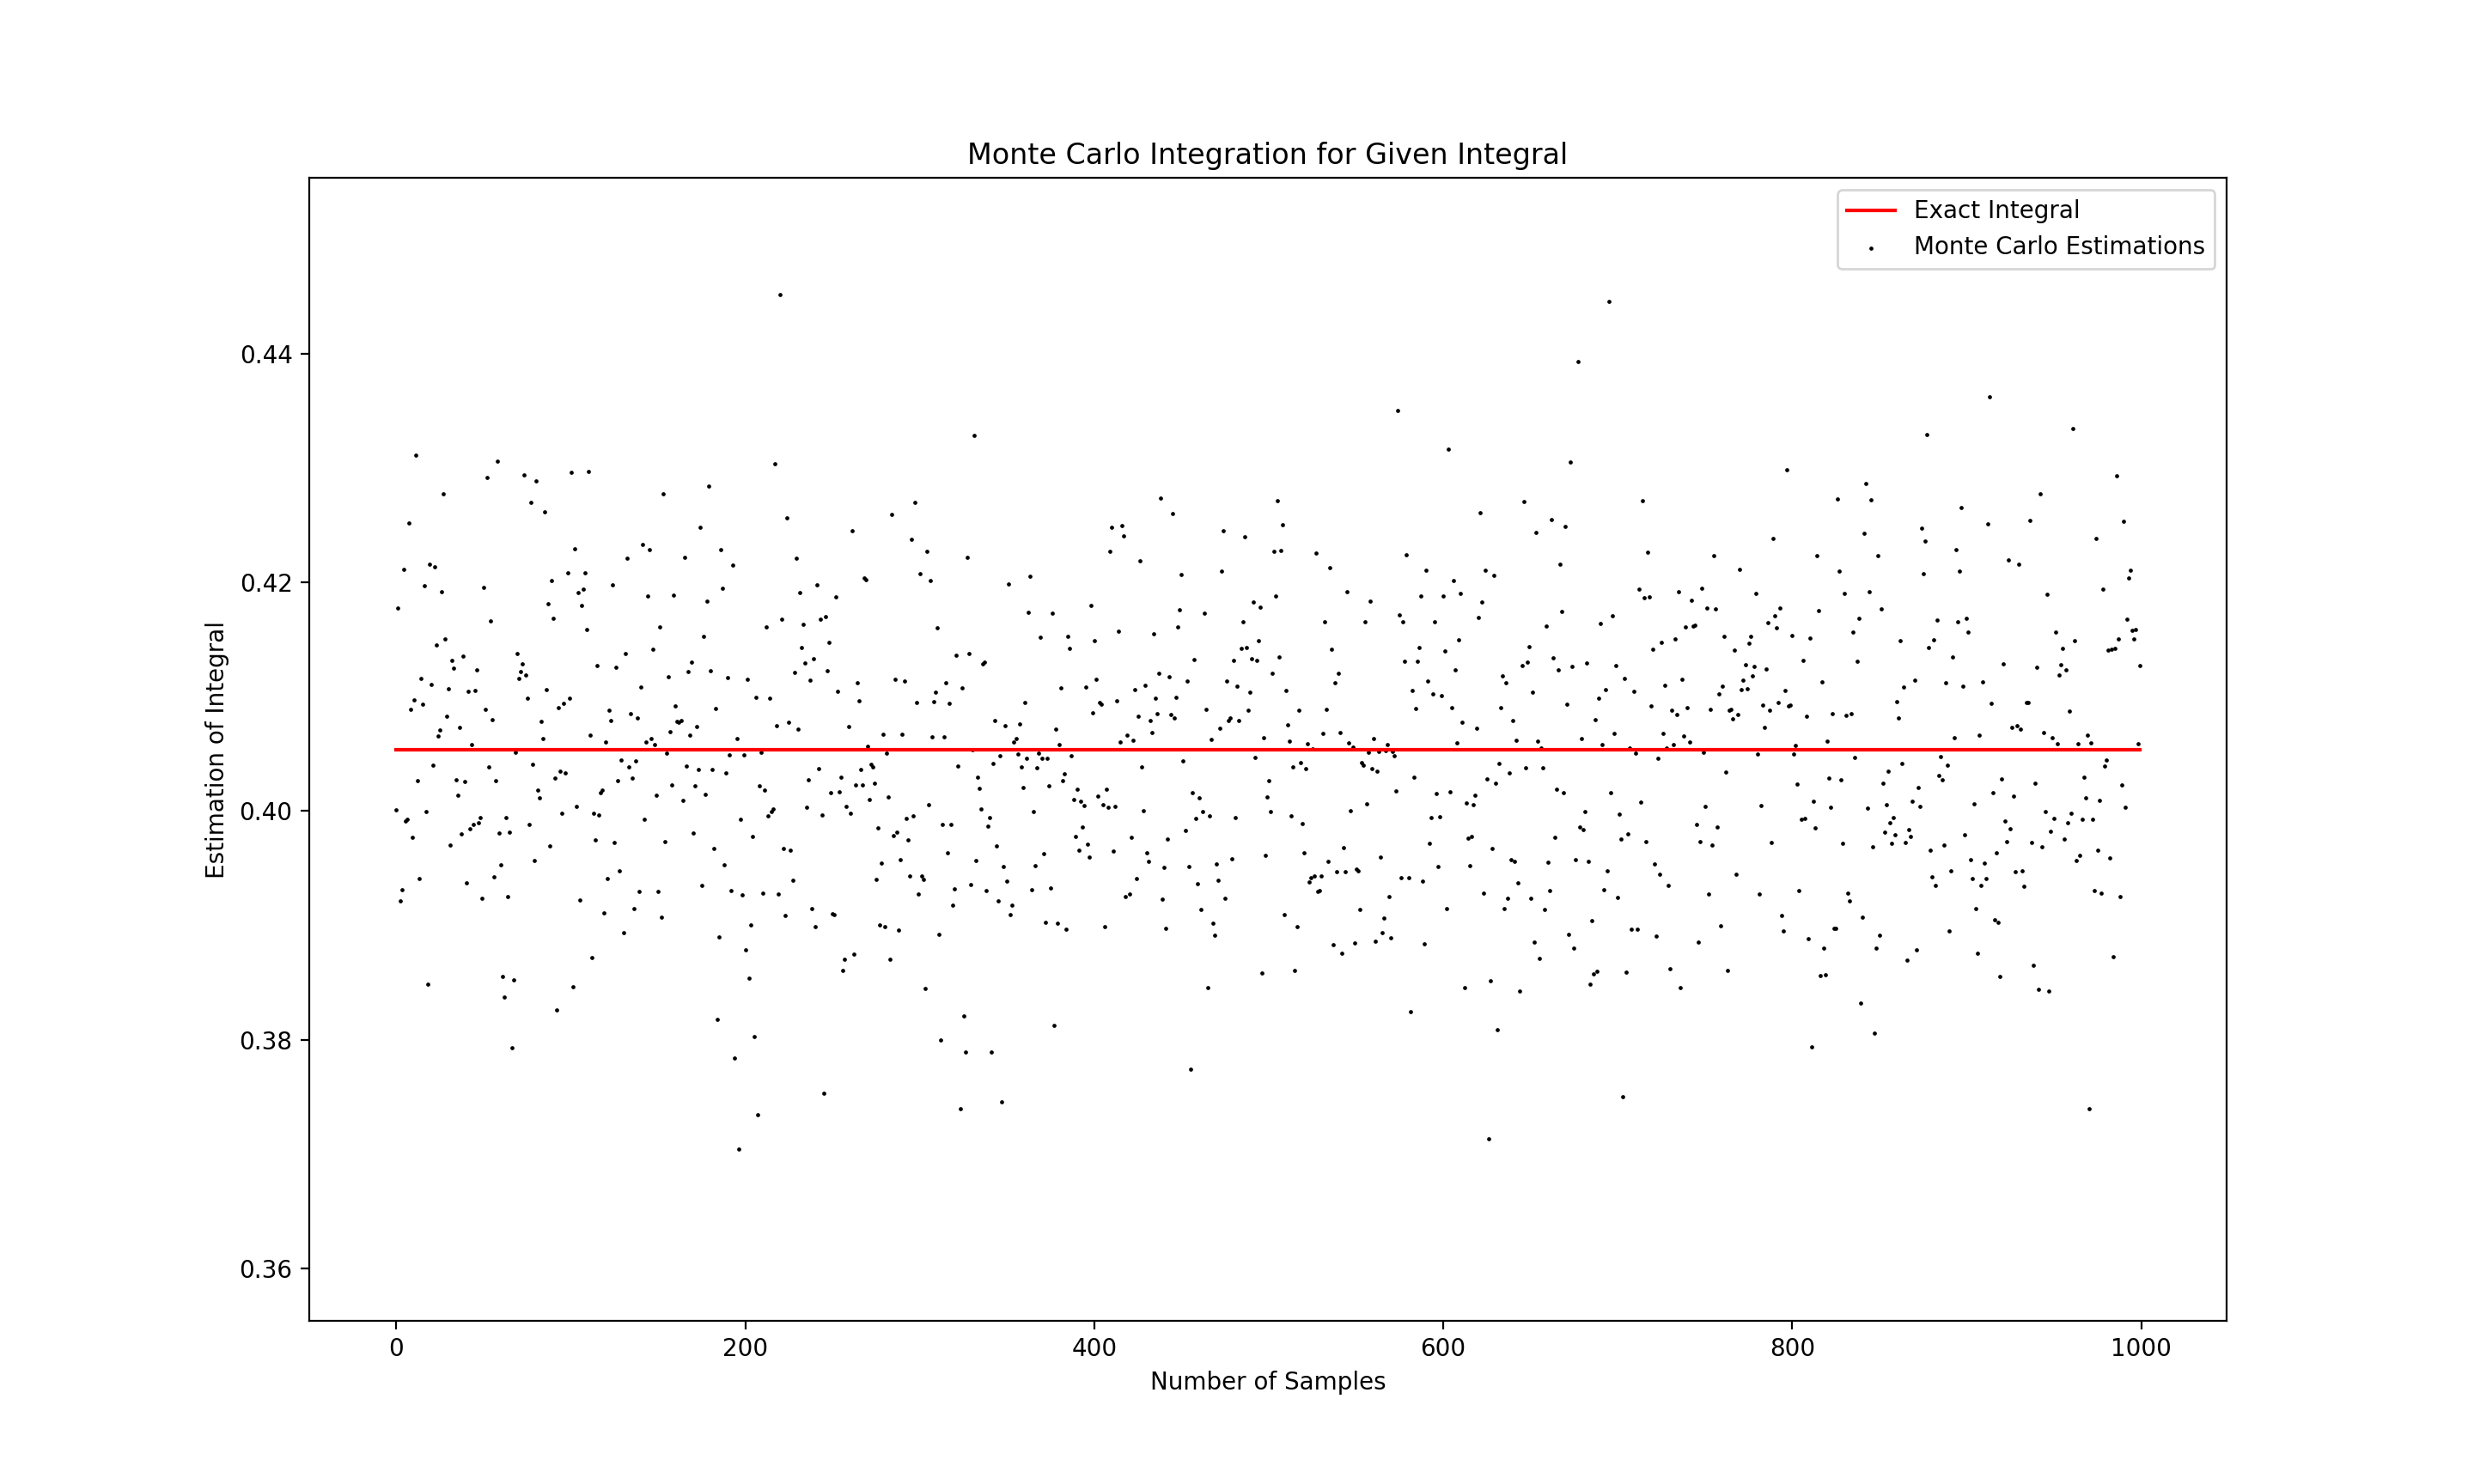
\includegraphics[scale=0.35, center]{HW1}
  \caption{Monte Carlo Integration for the Given Integral}
  \label{fig:mc_randomness}
\end{figure}


We notice that each estimation is within a small region above, below or exactly on the exact integral. To take this further, we could calculate the average of all $N = 1000$ estimates and plot the error versus $N$. This can be seen in Figure 6.

\begin{figure}[h!]
  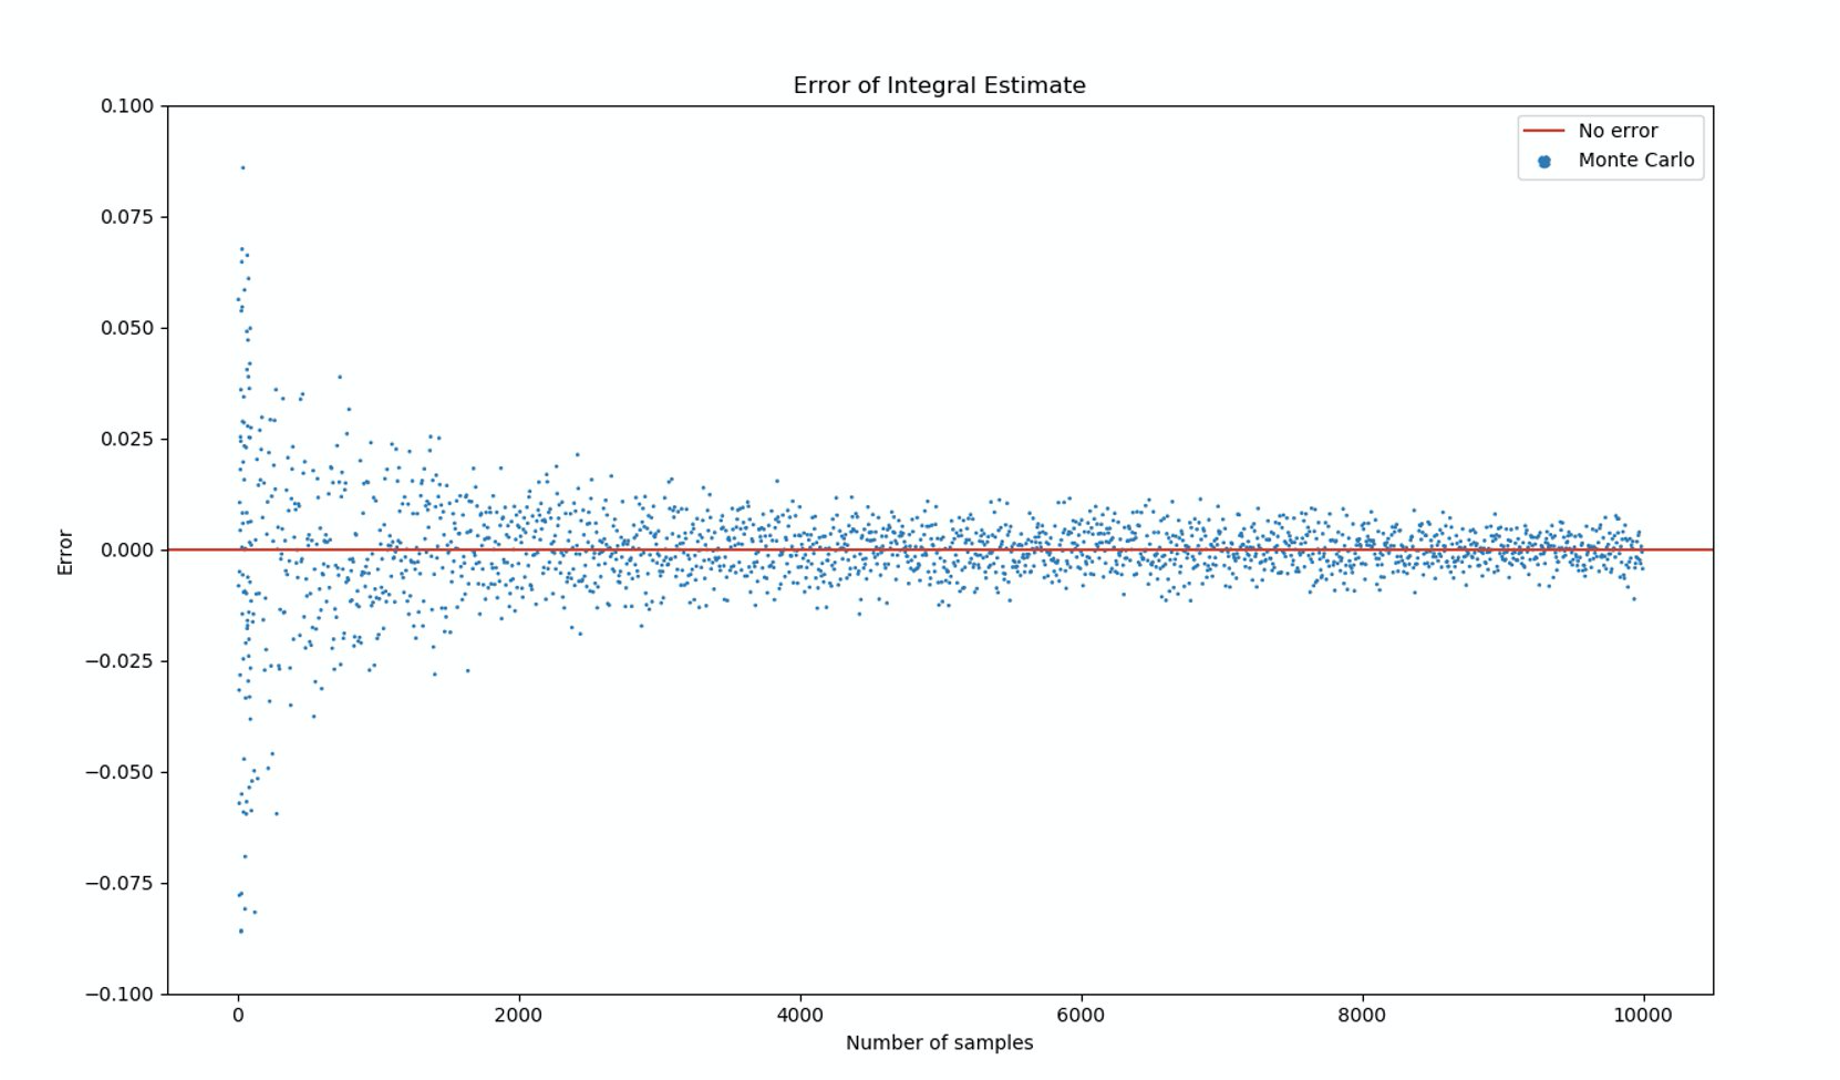
\includegraphics[scale=0.38, center]{Integral_Errors.png}
  \caption{Monte Carlo Integration for the Given Integral}
  \label{fig:mc_randomness}
\end{figure}

Although we see a convergence towards a 0 percent error, we still observe estimated values that lie within 0.025 of an error. 

We can extend the Monte Carlo error by comparing it against the Trapezium and Simpsons rule. 

\begin{figure}[h!]
  \includegraphics[scale=0.38, center]{Trap Simp Error.png}
  \caption{Monte Carlo Integration for the Given Integral}
  \label{fig:mc_randomness}
\end{figure}

To observe a difference between all three methods, we can plot on a loglog graph and observe any noticeable difference. 

\begin{figure}[h!]
  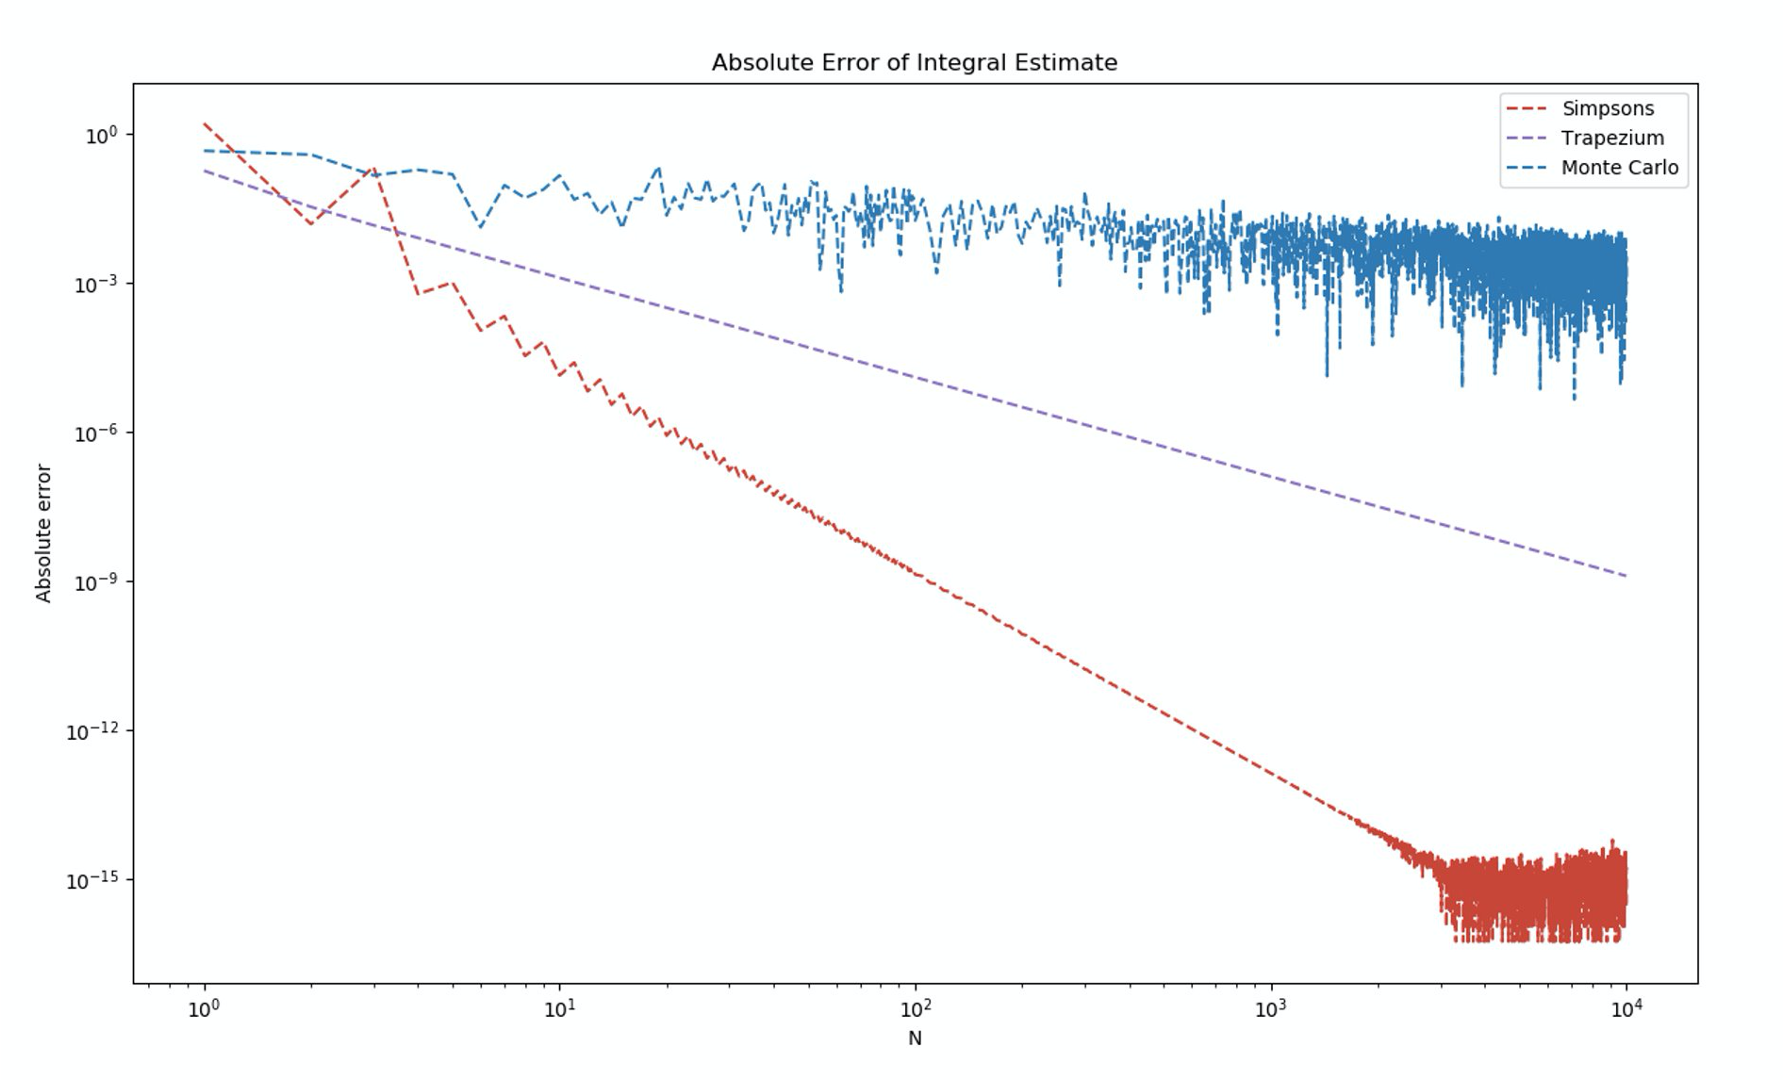
\includegraphics[scale=0.38, center]{loglog_errors.png}
  \caption{Monte Carlo Integration for the Given Integral}
  \label{fig:mc_randomness}
\end{figure}

In Figure 8, we observe that the Simpson's rule (red) converges to a 0 percent error fast than the Trapezium rule (purple). Both these methods also converge faster than the Monte Carlo estimations (blue). Thus, we conclude that for one dimension integration, Simpson's rule is the best followed by Trapezium and Monte Carlo methods. 

\subsection*{Homework Task 3}

Calculate the area of the unit circle by integrating the function,
\begin{align}
f =
\left\{
	\begin{array}{ll}
		1  & \mbox{if } x\textsubscript{1}^2 + x\textsubscript{2}^2 < 1 \\
		0 & \mbox{otherwise}
	\end{array}
\right.
\end{align}

\subsubsection*{Answer}

\end{document}

















